% ORIENTAÇÕES GERAIS------------------------------------------------------------
\chapter{ORIENTAÇÕES GERAIS}
\label{chap:orientacoesGerais}

Neste capítulo (que deve ser removido), são abordados detalhadamente os comandos para formatar o texto, criar listas, tabelas e figuras, inserir equações matemáticas, gerenciar referências bibliográficas.

% -------------------------------- FORMATAÇÃO DE TEXTO -------------------------------- %
\section{Formatação de Texto}
\label{sec:formatacaoTexto}

\begin{itemize}
\item \textbf{Negrito e Itálico:} Utilize os comandos \verb|\textbf{}| para negrito e \verb|\textit{}| para itálico. Exemplo: \textbf{texto em negrito} e \textit{texto em itálico}.

\item \textbf{Alinhamento do Texto:} Use \verb|\centering| para centralizar o texto, \verb|\raggedright| para alinhar à esquerda e \verb|\raggedleft| para alinhar à direita.

\item \textbf{Parágrafos e Espaçamento:} Para criar novos parágrafos, deixe uma linha em branco.

\item \textbf{Recuo de Parágrafo:} Se desejar evitar o recuo em um novo parágrafo, utilize o comando \verb|\noindent| no início.

\item \textbf{Quebras de Linha e Página:} Para quebrar linhas, utilize \verb|\\| e \verb|\newline|. Para quebrar páginas, utilize \verb|\newpage|.

\item \textbf{Comentários:} Utilize \verb|%| para fazer comentários no código LaTeX.
% Você pode deixar comentários para quem for ler seu código ou para servir como suas anotações ao longo do texto.

\item \textbf{Espaços:} Utilize \verb|~| para criar espaços não quebráveis e \verb|\hspace{}| para ajustar o espaçamento horizontal.

\end{itemize}


% -------------------------------- LISTAS -------------------------------- %

\section{Listas}
\label{sec:listas}

Em documentos \LaTeX, podemos criar listas não numeradas (\textit{bullets}) e numeradas utilizando os ambientes \verb|itemize| e \verb|enumerate|, respectivamente.

\subsection{Listas não numeradas}
\label{subsec:listasNaoNumeradas}

Para listas não numeradas, use o ambiente \verb|itemize| e marque cada item com \verb|\item|.

\textbf{Exemplo:}
\begin{verbatim}
\begin{itemize}
\item Item 1
\item Item 2
\end{itemize}
\end{verbatim}

\textbf{Resultado:}
\begin{itemize}
\item Item 1
\item Item 2
\end{itemize}

\subsection{Listas numeradas}
\label{subsec:listasNumeradas}

Para listas numeradas, use o ambiente \verb|enumerate| e marque cada item com \verb|\item|.

\textbf{Exemplo:}
\begin{verbatim}
\begin{enumerate}
\item Item 1
\item Item 2
\end{enumerate}
\end{verbatim}

\textbf{Resultado:}
\begin{enumerate}
\item Item 1
\item Item 2
\end{enumerate}


% CITAÇÕES ----------------------------------------------------------
\section{Citações}
\label{sec:citacoes}

Nesta seção, vamos abordar como fazer citações diretas e indiretas utilizando os comandos \LaTeX{} apropriados.

\subsection{Citação indireta}
\label{subsec:citacaoIndireta}

A citação indireta é a transcrição das ideias de um autor, utilizando suas próprias palavras, mas mantendo o sentido original. Para fazer uma citação indireta, utilize os comandos \verb|\cite{chave}| e \verb|\citeonline{chave}|, colocando entre as chaves o nome do autor ou o identificador da referência bibliográfica.

\textbf{Exemplos:}
\begin{itemize}
\item A epistemologia baseada na biologia considera que... \cite{Maturana2003}
\item Para \citeonline{Barbosa2004}, a citação indireta deve ser utilizada quando...
\end{itemize}

\subsection{Citação direta}
\label{subsec:citacaoDireta}

Quando o trecho citado é longo (4 ou mais linhas) deve-se usar um parágrafo específico para a citação, na forma de um texto recuado (4 cm da margem esquerda), com tamanho de letra menor e espaçamento entrelinhas simples. Exemplo de citação longa:
\\
\begin{citacao}
    Desse modo, opera-se uma ruptura decisiva entre a reflexividade filosófica, isto é a possibilidade do sujeito de pensar e de refletir, e a objetividade científica. Encontramo-nos num ponto em que o conhecimento científico está sem consciência. Sem consciência moral, sem consciência reflexiva e também subjetiva. Cada vez mais o desenvolvimento extraordinário do conhecimento científico vai tornar menos praticável a própria possibilidade de reflexão do sujeito sobre a sua pesquisa \cite[p.~28]{Silva2000}.
\end{citacao}

Para fazer a citação longa deve-se utilizar os seguintes comandos:
\begin{verbatim}
\begin{citacao}
<texto da citacao>
\end{citacao}
\end{verbatim}

No exemplo acima, para a chamada da referência o comando \verb|\cite[p.~28]{Silva2000}| foi utilizado, visto que os nomes dos autores não são parte do trecho citado. É necessário também indicar o número da página da obra citada que contém o trecho citado.


% SOBRE AS ILUSTRAÇÕES----------------------------------------------------------
\section{Referências Cruzadas}
\label{sec:referenciasCruzadas}

As referências cruzadas são uma funcionalidade essencial no \LaTeX{}, permitindo criar conexões automáticas entre diferentes partes do documento, como capítulos, seções, figuras, tabelas, equações e outros elementos numerados. Para utilizar referências cruzadas, é necessário incluir um rótulo (\textit{label}) em cada elemento que se deseja referenciar.

\subsection{Inserindo um Rótulo}
Para criar um rótulo, utilize o comando \verb|\label{nome}| no local desejado. O \verb|nome| é um identificador único que você atribui ao elemento. É recomendável utilizar nomes descritivos, como \verb|chap:orientacoesGerais| para um capítulo ou \verb|fig:exemplo| para uma figura. 

Exemplo:
\begin{verbatim}
\section{Listas}
\label{sec:listas}
\end{verbatim}

\subsection{Referenciando um Elemento}
Para fazer referência a um elemento previamente rotulado, utilize os comandos \verb|\ref{nome}| ou \verb|\autoref{nome}|. O comando \verb|\ref{nome}| simplesmente mostra o número do elemento referenciado, enquanto \verb|\autoref{nome}| adiciona automaticamente o tipo do elemento (como "Capítulo", "Figura", "Tabela", etc.) antes do número. Por exemplo, ao utilizar \verb|\autoref{fig:exemplo}|, o resultado será "Fig. 1".

Exemplo:
\begin{verbatim}
Na \autoref{sec:listas} são abordadas informações sobre listas no documento.
\end{verbatim}

Resultado: \\
"Na \autoref{sec:listas} são abordadas informações sobre listas no documento."

\subsection{Elementos com rótulos}
Aqui estão alguns elementos comuns que podem receber rótulos para referências cruzadas:

\begin{itemize}
\item Capítulos: \texttt{\textbackslash chapter\{...\}\textbackslash label\{chap:nome\}}
\item Seções: \texttt{\textbackslash section\{...\}\textbackslash label\{sec:nome\}}
\item Subseções: \texttt{\textbackslash subsection\{...\}\textbackslash label\{subsec:nome\}}
\item Figuras: \texttt{\textbackslash begin\{figure\}...\textbackslash caption\{...\}\textbackslash label\{fig:nome\}\textbackslash end\{figure\}}
\item Tabelas: \texttt{\textbackslash begin\{table\}...\textbackslash caption\{...\}\textbackslash label\{tab:nome\}\textbackslash end\{table\}}
\item Equações: \texttt{\textbackslash begin\{equation\}...\textbackslash label\{eq:nome\}\textbackslash end\{equation\}}
\end{itemize}
\vspace{0.5cm}
Com o uso adequado de rótulos e referências cruzadas, você pode criar um documento bem estruturado e de fácil navegação no \LaTeX{}. 



% FIGURAS-----------------------------------------------------------------------
\section{Figuras}
\label{sec:figuras}

Exemplo de como inserir a \autoref{fig:figura-exemplo-1}. Também pode ser usado \cref{fig:figura-exemplo-1}. As figuras aparecem automaticamente na lista de figuras. Os arquivos das imagens devem ser armazenados no diretório de "/dados".

\begin{figure}[!htb]
    \centering
    \caption{Exemplo de Figura}
    \sbox0{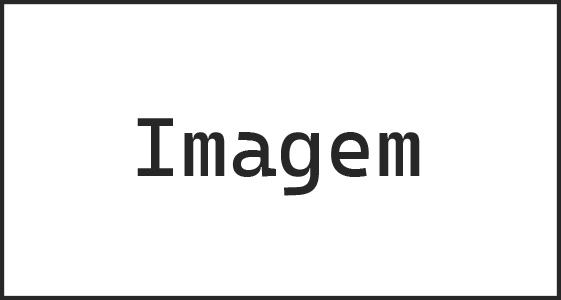
\includegraphics[width=0.5\textwidth]{./dados/figuras/figura1}}% measure width
    \begin{minipage}{\wd0}
    \usebox0
        \label{fig:figura-exemplo-1}
        \fonte{\citeonline{IRL2014}}
    \end{minipage}
\end{figure}



% QUADROS E TABELAS---------------------------------------------------------------
\section{Quadros e tabelas}
\label{sec:tabelas}

Exemplo de como inserir o \autoref{qua:quadro-exemplo1} e a \autoref{tab:tabela-exemplo1} (ou \cref{tab:tabela-exemplo1}). Ambos aparecem automaticamente nas suas respectivas listas.
Ambos os elementos (Quadros e Tabelas) devem ser criados em arquivos separados para facilitar manutenção e armazenados no diretório de "/dados".

\begin{quadro}[!htb]
    \centering
    \caption{Campo elétrico produzido por distribuição esférica de carga.\label{qua:quadro-exemplo1}}
    \begin{tabular}{|p{5cm}|p{4.8cm}|p{4.8cm}|}
        \hline
        \textbf{Distribuição de cargas} & \textbf{Ponto em campo elétrico} & \textbf{Módulo do campo elétrico} \\
        \hline
        Carga $q$ sobre a superfície de uma esfera condutora com o raio $R$. & 
        
        Fora da esfera, $r > R$ \newline \newline
        Dentro da esfera, $r < R$ & 
        
        $E = \frac{1}{4\pi\varepsilon_0} \frac{Q}{r^2}$ \newline \newline
        $E = 0$
        \\
        \hline
    \end{tabular}
    \fonte{\citeonline{young}.}
\end{quadro}


A diferença entre quadro e tabela está no fato que um quadro é formado por linhas horizontais e verticais. Deve ser utilizado quando o conteúdo é majoritariamente não-numérico. Uma tabela é formada apenas por linhas verticais, e deve ser utilizada quando o conteúdo é majoritariamente numérico.

\begin{table}[!htb]
    \centering
    \caption{Algumas propriedades elétricas do cobre e do silício. \label{tab:tabela-exemplo1}}
    \begin{tabularx}{\textwidth}{lcc}
        \toprule
            Propriedade                                            & Cobre & Silício      \\ 
        \midrule
            % Tipo de material                                       & Metal & Semicondutor \\
            Densidade de portadores de carga, $m^{-3}$             & $\mathrm{8,49} \times 10^{28}$ & $\mathrm{1} \times 10^{16}$     \\
            Resistividade, $\Omega \cdot m$                        & $\mathrm{1,69} \times 10^{-8}$  & $\mathrm{2,5} \times 10^{3}$   \\
            Coeficiente de temperatura da resistividade, $K^{-1}$  & $\mathrm{+4,3} \times 10^{-3}$  & $\mathrm{-70} \times 10^{-3}$  \\ 
        \bottomrule
    \end{tabularx}
    \fonte{\citeonline{halliday}.}
\end{table}

% EQUAÇÕES-----------------------------------------------------------------------
\section{Equações}
\label{sec:equacoes}

Exemplo de como inserir a \autoref{eq:equacao-exemplo1} e a \cref{eq:equacao-exemplo2} no corpo do texto. Observe que foram utilizadas duas formas distintas para referenciar as equações. O comando \verb|\ref{nome}| também é válido para exibir apenas o número da equação.

\begin{equation}
    \label{eq:equacao-exemplo1}
    f(x) = \frac{a_0}{2} + \sum_{n=1}^{\infty} \left[a_n \cos{ \left( \frac{ n\pi x}{L} \right) }  +  b_n  \: \mathrm{sen}{ \left( \frac{ n\pi x}{L} \right) }     \right]
    ,
\end{equation}

\begin{equation}
    \phi_E  = \int \limits_{A} \Vec{E_1}\cdot (-\Hat{n}) \, dA'\ + \int \limits_{A} \Vec{E_2}\cdot \Hat{n} \, dA'\
    \label{eq:equacao-exemplo2}
\end{equation}

% ALGORITMOS-----------------------------------------------------------------------
\section{Algoritmos}
\label{sec:algoritmos}

Exemplo de como inserir um algoritmo. Para inserção de algoritmos utiliza-se o pacote {\ttfamily algorithm2e} que já está devidamente configurado dentro do template.

Os algoritmos devem ser criados em arquivos separados para facilitar manutenção e armazenados no diretório de "/dados". \\
\begin{algorithm}
    \caption{Algoritmo de Fibonacci Recursivo: $O(2^n)$}
    \KwIn{inteiro não negativo $n$}
    \KwOut{valor do $n$-ésimo número de Fibonacci $F(n)$}
    \If{$n \leq 1$}{
        \Return $n$
    }
    \Return $F(n-1) + F(n-2)$
\end{algorithm}


% SOBRE AS REFERÊNCIAS BIBLIOGRÁFICAS-------------------------------------------------------
\section{Referências bibliográficas}
\label{sec:referenciasBibliograficas}

A bibliografia é feita no padrão \textsc{Bib}\TeX{}. As referências são colocadas em um arquivo separado. Neste template as referências são armazenadas no arquivo "base-referencias.bib".

Existem diversas categorias documentos e materiais componentes da bibliografia. A classe abn\TeX{} define as seguintes categorias (entradas):

\begin{verbatim}
@book
@inbook
@article
@phdthesis
@mastersthesis
@monography
@techreport
@manual
@proceedings
@inproceedings
@journalpart
@booklet
@patent
@unpublished
@misc
\end{verbatim}

Cada categoria (entrada) é formatada pelo pacote \citeonline{abnTeX22014d} de uma forma específica. Algumas entradas foram introduzidas especificamente para atender à norma \citeonline{NBR6023:2002}, são elas: \verb|@monography|, \verb|@journalpart|,\verb|@patent|. As demais entradas são padrão \textsc{Bib}\TeX{}. Para maiores detalhes, refira-se a \citeonline{abnTeX22014d}, \citeonline{abnTeX22014b}, \citeonline{abnTeX22014c}.
